\documentclass[12pt]{article}
\usepackage[left=1in,right=1in,top=1in,bottom=1in]{geometry}%
\let\bibsection\relax
\usepackage{amsrefs}
\usepackage{amsmath}
\usepackage{enumerate}
\usepackage{amssymb}                
\usepackage{amsmath}                
\usepackage{amsfonts}
\usepackage{amsthm}
\usepackage{bbm}
\usepackage{float}
\usepackage{mathtools}
\usepackage{graphicx,epsfig}
\usepackage{hyperref}

\RequirePackage{xcolor}[2.11]
\colorlet{siaminlinkcolor}{green!50!black}
\colorlet{siamexlinkcolor}{red!50!black}
\colorlet{siamreviewcolor}{black!50}
\hypersetup{
  hidelinks = true,
  colorlinks = false,
  allcolors = siaminlinkcolor,
  urlcolor = siamexlinkcolor,
}

% default SIAM options for cleveref

\usepackage[capitalize,nameinlink]{cleveref}
% Per SIAM Style Manual, "section" should be lowercase
\crefname{section}{section}{sections}
\crefname{subsection}{subsection}{subsections}
\Crefname{section}{Section}{Sections}
\Crefname{subsection}{Subsection}{Subsections}

% Per SIAM Style Manual, "Figure" should be spelled out in references
\Crefname{figure}{Figure}{Figures}

% Per SIAM Style Manual, don't say equation in front on an equation.
\crefformat{equation}{\textup{#2(#1)#3}}
\crefrangeformat{equation}{\textup{#3(#1)#4--#5(#2)#6}}
\crefmultiformat{equation}{\textup{#2(#1)#3}}{ and \textup{#2(#1)#3}}
{, \textup{#2(#1)#3}}{, and \textup{#2(#1)#3}}
\crefrangemultiformat{equation}{\textup{#3(#1)#4--#5(#2)#6}}%
{ and \textup{#3(#1)#4--#5(#2)#6}}{, \textup{#3(#1)#4--#5(#2)#6}}{, and \textup{#3(#1)#4--#5(#2)#6}}

% But spell it out at the beginning of a sentence.
\Crefformat{equation}{#2Equation~\textup{(#1)}#3}
\Crefrangeformat{equation}{Equations~\textup{#3(#1)#4--#5(#2)#6}}
\Crefmultiformat{equation}{Equations~\textup{#2(#1)#3}}{ and \textup{#2(#1)#3}}
{, \textup{#2(#1)#3}}{, and \textup{#2(#1)#3}}
\Crefrangemultiformat{equation}{Equations~\textup{#3(#1)#4--#5(#2)#6}}%
{ and \textup{#3(#1)#4--#5(#2)#6}}{, \textup{#3(#1)#4--#5(#2)#6}}{, and \textup{#3(#1)#4--#5(#2)#6}}

% Make number non-italic in any environment.
\crefdefaultlabelformat{#2\textup{#1}#3}

% useful macros
\def\noi{\noindent}
\def\T{{\mathbb T}}
\def\R{{\mathbb R}}
\def\N{{\mathbb N}}
\def\C{{\mathbb C}}
\def\Z{{\mathbb Z}}
\def\P{{\mathbb P}}
\def\E{{\mathbb E}}
\def\Q{\mathbb{Q}}
\def\ind{{\mathbb I}}

\def\calH{{\mathcal H}}
\def\calE{{\mathcal E}}
\def\calQ{{\mathcal Q}}
\def\calL{{\mathcal L}}
\def\calI{{\mathcal I}}

\DeclareMathOperator{\spn}{span}
\DeclareMathOperator{\ran}{ran}

\newtheorem{lemma}{Lemma}
\newtheorem{theorem}{Theorem}
\newtheorem{corollary}{Corollary}
\newtheorem{definition}{Definition}
\newtheorem{hypothesis}{Hypothesis}
\newtheorem{remark}{Remark}

\graphicspath{ {images/} }

\title{Multi-pulse solitary waves in a fourth-order NLS equation}

\begin{document}

\maketitle

\section{Introduction}
It has been nearly 50 years since the discovery by Zakharov and Shabat \cite{Zak72} of the integrability of the Nonlinear Schr\"odinger equation (NLS) and the corresponding soliton solutions and 40 years of the first experimental demonstration by Mollenauer, Stolen and Gordon of optical solitons propagating in fibers \cite{Moll80}. At the most fundamental level, the realization of the soliton represents the balance of chromatic second order dispersion and the Kerr self-focusing nonlinearity. The robustness of the soliton opened new directions both in the theoretical and experimental fronts that continue to this day. On the other hand, as better fibers were built and with technological advances leading to the invention of photonic crystal fibers, that in particular enabled the engineering of the dispersion resulting on new discoveries such as supercontinuum generation realized in regimes far from the NLS equation.   
In this vein, a recent experimental work in silicon photonic
crystal waveguides produced for the first time what is now known as pure quartic solitons (PQS) \cite{BlancoPQS}; the term reflects that for this waveguide the leading dispertion term is fourth order. A few recent results both on theory and experiments have followed \cite{Tam2019, Tam2020} that on the theoretical side include existence and linear stability properties. Our results presented here provide a more rigorous study of PQS including for the first time the existence of pulse trains which we suggest can support the creation of such trains in laser cavities.

\noindent
After a brief background, we first present results on the existence and stability of solitons in the more general case where both second and fourth order dispersion are accounted for. This results include the particular case of PQS. The second part of the paper proves the existence of (in phase and out of phase) pulse trains, which in turn are unstable. Numerical examples are presented in the last section.


\section{Background}

The following fourth-order generalization of the nonlinear Schr{\"o}dinger equation (NLS)
\begin{equation}\label{NLS4}
i u_t + \frac{\beta_4}{24}u_{xxxx} - \frac{\beta}{2}u_{xx} + \gamma |u|^2 u = 0,
\end{equation}
was recently investigated in \cite{Tam2020} in a study of the properties of solitary wave solutions under a combination of second- and fourth-order dispersion. (We use the independent variables $(t, x)$ in place of $(z, \tau)$ in \cite{Tam2020}). Ordinary NLS solitons are solutions when $\beta_2 < 0$ and $\beta_4 = 0$. Pure quartic solitons (PQSs) occur when $\beta_2 = 0$ and $\beta_4 < 0$, i.e. $u(x,t)$ satisfies the equation
\begin{equation}\label{PQSeq}
i u_t + \frac{\beta_4}{24}u_{xxxx} + \gamma |u|^2 u = 0.
\end{equation}
Unlike ordinary NLS solitons, PQSs have oscillatory, exponentially decaying tails. There has been much recent interest in PQSs due to the their discovery in experimental media by Blanco-Redondo et al. in 2016 \cite{BlancoPQS}. The existence and spectral stability of PQS solutions to \cref{PQSeq} was shown in \cite{Tam2019}, and the existence of solitary wave solutions to the more general equation \cref{NLS4} in terms of the parameters $\beta_2$ and $\omega$ is given in \cite{Tam2020}.

Real-valued, standing wave solutions, i.e. solutions of the form $e^{i \omega t} u(x)$, satisfy the ODE 
\begin{equation}\label{standingwavereal}
\frac{\beta_4}{24}u_{xxxx} - \frac{\beta}{2}u_{xx} + \gamma u^3 - \omega u = 0
\end{equation}
For PQSs, equation \cref{standingwavereal} can be written in parameter-free form by using the rescaling $u(x; \omega) = \sqrt{\frac{\omega}{\gamma}}\tilde{u}(\omega^{1/4}x)$ to obtain the equation
\begin{equation}\label{PQSparfree}
\frac{\beta_4}{24}\tilde{u}_{xxxx} + \tilde{u}^3 - \tilde{u} = 0
\end{equation}
Observe that the power or photon number of PQS scale as $\omega^{3/4}$ compared to the $\omega^{1/2}$ scaling of classical (NLS) solitons. A more general rescaling \cite[Section VI]{Tam2020} transforms equation \cref{standingwavereal} into the one-parameter equation
\begin{equation}\label{NLS4onepar}
\tilde{u}_{xxxx} + 2 \sigma \tilde{u}_{xx} +  \tilde{u} - |\tilde{u}|^2 \tilde{u} = 0,
\end{equation}
where 
\[
\sigma = \sqrt{\frac{3}{2 \omega |\beta_4| }}\beta_2
\]
is a non-dimensional parameter characterizing the relative strengths of the quadratic and quartic dispersion terms.

For ordinary NLS, an analytic solution is known. For $\beta_4 < 0$ and $\beta_2 < 0$, an analytic solution has also been obtained for $\omega = \frac{24 \beta_2^2}{25 |\beta_4|}$ \cite{KarllsonHook}. 

\section{Mathematical setup}

Equation \cref{NLS4} can be written in Hamiltonian form as 
\begin{equation}\label{NLSHam}
\frac{\partial u}{\partial t} = J \calE'(u(t)),
\end{equation}
where $J = -i$ and the energy $\calE$ is given by
\begin{equation}\label{defH}
\calE(u) = \frac{1}{2} \int_{-\infty}^\infty \left( \frac{\beta_4}{24}|u_{xx}|^2 + \frac{\beta_2}{2}|u_{x}|^2 + \frac{\gamma}{2} |u|^4 \right) dx
\end{equation}
The energy $\mathcal{E}$ is invariant under the complex rotation group $T(\theta)$, given by $T(\theta)u = e^{i\theta}u$. The corresponding conserved quantity, often called the charge \cite[Section 6.C]{Grillakis1987}, is given by
\begin{equation}\label{defQ}
\mathcal{Q}(u) = -\frac{1}{2} \int_{\infty}^\infty |u|^2 dx.
\end{equation}

We make the following hypothesis regarding the well-posedness of \cref{NLSHam}, which is the same as \cite[Assumption 1]{Grillakis1987}.

\begin{hypothesis}\label{hyp:wp}
For each initial condition $u_0$ there exists $T > 0$ depending only on $K$, where $\|u_0\| \leq K$, such that the PDE \cref{NLSHam} has a solution $u(t)$ on $[0, T]$ with $u(0) = u_0$.
\end{hypothesis}

Standing waves are solutions of the form $T(\omega t) u$, where $u$ is independent of $t$. A standing wave solution satisfies the standing wave equation $\calE'(u) - w \calQ'(u) = 0$ \cite[2.15]{Grillakis1987}. Since $\calQ'(u) = -u$, standing waves satisfy the equation
\begin{equation}\label{standingwaveeq}
\calE'(u) + w u = 0,
\end{equation}
which can be written as
\begin{equation}\label{standingwaveeq2}
\frac{\beta_4}{24}u_{xxxx} - \frac{\beta_2}{2}u_{xx} + \gamma |u|^2 u - \omega u = 0
\end{equation}

The following theorem gives criteria for the existence of real-valued solitary wave solutions to \cref{standingwaveeq2} in terms of the parameters $\beta_2$, $\beta_4$ and $\omega$. We only consider $\beta_4 < 0$, since that is the physically relevant regime.

\begin{theorem}\label{theorem:solitonexist}
Let $\beta_4 < 0$, and define
\begin{equation}\label{omegac}
\omega_c = \frac{3}{2} \frac{\beta_2^2}{|\beta_4|}.
\end{equation}
Then for either (i) $\omega > \omega_c$, or (ii) $0 < \omega < \omega_c$ and $\beta_2 < 0$, 
there exists a real-valued, symmetric, exponentially localized solution $\phi(x; \omega) \in H^2(\R) \cap C^5(\R)$ of the standing wave equation \cref{standingwaveeq2}. 
\begin{proof}
The existence result follows from \cite{Groves1998}, which uses the mountain pass lemma and the concentration-compactness principle. Exponential localization follows from the stable manifold theorem.
\end{proof}
\end{theorem}

\begin{remark}
For $\omega > \omega_c$, it follows from \cite{Groves1998} that there exists a countably infinite family of distinct solitary-wave solutions. These are the multi-pulse solutions we will construct below. We also note that for $\beta_2 = 0$, $\omega_c = 0$, thus pure quartic solitary waves exist for all $\omega > 0$.
\end{remark}

We make the following standard smoothness assumption (see, for example, \cite[Assumption 2]{Grillakis1987}) concerning the solutions $u(x; \omega)$ to \cref{standingwavereal}.

\begin{hypothesis}\label{hyp:smoothmap}
The map $\omega \mapsto \phi(x; \omega)$ from $\calI$ to $H^2(\R)$ is $C^1$, where $\calI$ is the interval for which the primary pulse solution $\phi(x; \omega)$ exists by \cref{theorem:solitonexist} for all $\omega \in \calI$ for a given $\beta_4 < 0$ and $\beta_2$.
\end{hypothesis}

Define the scalar
\begin{equation}
d(\omega) = \calE(\phi(\omega)) - \omega\calQ(\phi(\omega)).
\end{equation}
By \cite[(2.21)]{Grillakis1987},
\begin{align}\label{ddoubleprime}
d''(\omega) = \langle \calQ'(\phi(x; \omega)), \partial_\omega \phi(x; \omega) \rangle
= \int_{-\infty}^\infty \phi(x; \omega) \partial_\omega \phi(x; \omega) dx
\end{align}
By \cite[Theorem 3.5]{Grillakis1987}, the standing wave $\phi(x; \omega)$ is orbitally stable if $d''(\omega) > 0$. This quantity is easy to compute numerically, and we take this stability criterion as a hypothesis.

\begin{hypothesis}\label{hyp:dccpos}
For each $\omega$ such that a primary pulse solution $\phi(x; \omega)$ exists by \cref{theorem:solitonexist}, $d''(\omega) > 0$.
\end{hypothesis}

Fix $\beta_4 < 0$ and $\beta_2 \in \R$, and choose $\omega > 0$ such that the primary pulse solution $\phi(x) = \phi(x; \omega)$ exists. The linearization of the PDE \cref{NLS4} about $\phi$ is the linear operator $\calL(\phi)$
\begin{align}\label{defLphi}
\calL(\phi) = 
\begin{pmatrix}
0 & \calL^-(\phi) \\
-\calL^+(\phi) & 0
\end{pmatrix},
\end{align}
where
\begin{align*}
\calL^-(\phi) &= -\frac{\beta_4}{24} \partial_{xxxx} + \frac{\beta_2}{2} \partial_{xx} + \omega - \gamma \phi^2 \\
\calL^+(\phi) &= -\frac{\beta_4}{24} \partial_{xxxx} + \frac{\beta_2}{2} \partial_{xx} + \omega - 3 \gamma \phi^2
\end{align*}
It is straightforward to verify that 
\begin{align*}
\calL^-(\phi) \phi &= 0 \\
\calL^+(\phi) \partial_x \phi &= 0 \\
\calL^+(\phi)(-\partial_\omega \phi) &= \phi
\end{align*}
Furthermore, since $\calL^-(\phi)$ is self-adjoint and $\phi' \perp \ker \calL^-(\phi)$, there exists $z$ such that $\calL^-(\phi) z = \phi'$. For the second-order NLS equation ($\beta_4 = 0, \beta_2 \neq 0$), $z = \frac{1}{2 \beta_2} x \phi$. Thus $\calL(\phi)$ has a kernel with (at least) algebraic multiplicity 4 and geometric multiplicity 2, i.e.
\begin{equation}\label{Lphikernel}
\begin{aligned}
\calL(\phi)\begin{pmatrix}0 \\ \phi \end{pmatrix} &= 0, 
\calL(\phi)\begin{pmatrix} \partial_\omega \phi \\ 0 \end{pmatrix} = \begin{pmatrix}0 \\ \phi \end{pmatrix} \\
\calL(\phi)\begin{pmatrix}\partial_x\phi \\ 0 \end{pmatrix} &= 0, 
\calL(\phi)\begin{pmatrix} 0 \\ z \end{pmatrix} = \begin{pmatrix}\partial_x\phi \\ 0 \end{pmatrix} 
\end{aligned}
\end{equation}

To find the essential spectrum, which is independent of $\phi$ and only depends on the background state, the linear operator $\calL(\phi)$ is exponentially asymptotic to $\calL(0)$, given by
\begin{align}\label{defL0}
\calL(0) = 
\begin{pmatrix}
0 & \calL_0 \\
-\calL_0 & 0
\end{pmatrix}, \quad
\calL_0 = -\frac{\beta_4}{24} \partial_{xxxx} + \frac{\beta_2}{2} \partial_{xx} + \omega
\end{align}.
Thus the eigenvalue problem $\calL(0) v = \lambda v$ is equivalent to $(\calL_0 + \lambda^2)p = 0$. By \cite[Theorem 3.1.13]{Kapitula2013}, the essential spectrum is given by the curves
\begin{align*}
\left[ -\frac{\beta_4}{24} (ik)^4 + \frac{\beta_2}{2}(ik)^2 + \omega \right]^2 + \lambda^2 &= 0 && k \in \R,
\end{align*}
from which it follows that
\begin{align*}
\sigma_{ess} = \left\{ \pm i \left( -\frac{\beta_4}{24}k^4 - \frac{\beta_2}{2}k^2 + \omega \right) : k \in \R \right\}
\end{align*}
If $\beta_4 < 0$ and $\beta_2 \leq 0$, the essential spectrum is purely imaginary and given by 
\begin{equation}\label{PQSessspec}
\sigma_{ess} = \{ k i : k \in \R, |k| \geq \omega \},
\end{equation}
which is bounded away from the origin and independent of $\beta_4$ and $\beta_2$. If $\beta_4 < 0$, $\beta_2 > 0$, and $\omega > \omega_c$, the essential spectrum is also purely imaginary and given by 
\begin{equation}\label{essspec2}
\sigma_{ess} = \{ k i : k \in \R, |k| \geq (\omega - \omega_c) \},
\end{equation}
which does depend on $\beta_4$ and $\beta_2$, but is bounded away from the origin.

By the stability assumption in \cref{hyp:dccpos}, no element of the spectrum of $\calL(\phi)$ can have a positive real part. Since the PDE \cref{NLS4} is Hamiltonian, all elements of the spectrum of $\calL(\phi)$ must come in quartets $\pm \alpha \pm \beta i$, thus the spectrum of $\calL(\phi)$ is contained in the imaginary axis. For pure quartic solitary waves, there is an additional pair of imaginary eigenvalues located right before the essential spectrum boundary (approximately $\pm 0.9972 \omega i$) \cite{Tam2019}, which corresponds to an internal mode of the solitary wave. For $\beta_2 \neq 0$, there can be multiple pairs of internal mode eigenvalues (an example of two pairs internal mode eigenvalues is shown in \cite[Figure 9]{Tam2020}). These internal mode eigenvalues must be purely imaginary and will have no bearing on our analysis.

\subsection{Generalization to higher order solitons}
In a recent conference presentation \cite{Runge2020}, it was shown this by incorporating an intracavity programmable pulse-shaper in a mode-locked fiber laser one can manipulate the net-cavity dispersion by applying a phase to the pulse so that to leading order, the stationary pulse generated is modeled by the higher-order NLS equation:

\begin{equation}\label{HONLS}
-(i)^k\frac{d^k u}{dx^k}+ \omega u - \gamma u^3 = 0,
\end{equation}

\noindent
where k = 6,8,10,... (even), whose profile satisfy the scaling 
$u(x; \omega) = \sqrt{\frac{\omega}{\gamma}}\tilde{u}
(\omega^{1/k}x)$.

\section{Existence of multi-pulse solitary waves}

Let $\beta_4 < 0$. Using a spatial dynamics approach, we rewrite equation \cref{standingwavereal} by letting $U = (u_1, u_2, u_3, u_4) = (u, \partial_x u, \partial_x^2 u, \frac{\beta_4}{24} \partial_x^3 u)$ to get the first order system
\begin{equation}\label{Fsystem}
U' = F(U) = \begin{pmatrix}
u_2 \\ u_3 \\ \frac{24}{\beta_4} u_4 \\ \omega u_1 - \gamma u_1^3.
\end{pmatrix}
\end{equation}
Equation \cref{Fsystem} has a conserved quantity
\begin{equation}\label{FsystemH}
H(u_1, u_2, u_3, u_4) = -u_4 u_2 - \frac{1}{2} u_3^2 + \frac{\beta_2}{4}u_2^2 - \frac{\gamma}{4} u_1^4 + \frac{1}{2}\omega u_1,
\end{equation}
which we obtain by multiplying \cref{standingwavereal} by $u_x$ and integrating once, where the first term on the RHS is also integrated by parts. $F(0) = 0$, and the characteristic polynomial of $DF(0)$ is
\[
p(t) = t^4 - 12\frac{\beta_2}{\beta_4} t^2 - \frac{24}{\beta_4}\omega,
\]
which has a quartet of complex eigenvalues $\pm a \pm b i$ when $\omega > \omega_c$. Thus for $\omega > \omega_c$, 0 is a hyperbolic equilibrium of \cref{Fsystem} with two-dimensional stable and unstable manifolds. From a spatial dynamics perspective, the primary pulse solution is a homoclinic orbit connecting this equilibrium point to itself.  For $\omega > \omega_c$, the exponentially localized pulse solution corresponding to this homoclinic orbit will have oscillatory tails. In particular, this is always the case for PQSs. 

We have the following result concerning the existence of multi-pulse solutions, which follows immediately from \cite[Theorem~3.6]{SandstedeStrut}. The main difference is that neighboring pulses in the multi-pulse can be either in-phase or out-of-phase. 

\begin{theorem}\label{theorem:multiexist}
Assume \cref{hyp:wp}, \cref{hyp:smoothmap}, and \cref{hyp:dccpos}, and fix $\omega > \omega_c$. Let $\phi(x)$ be the real-valued, symmetric, exponentially localized primary pulse solution to \cref{standingwavereal} from \cref{theorem:solitonexist}, and let $U(x) = (\phi(x), \partial_x \phi(x), \partial_x^2 \phi(x), \partial_x^3 \phi(x))$ be the corresponding homoclinic orbit solution to \cref{Fsystem}. Let $\pm a \pm bi$ be the eigenvalues of $DF(0)$, with $a > 0$ and $b > 0$. Then for any 
\begin{itemize}
\item $n \geq 2$
\item Sequence of nonnegative integers $\{ k_1, \dots, k_{n-1} \}$, with at least one of the $k_j \in \{0, 1 \}$
\item Sequence of phase parameters $\{ \theta_1, \dots, \theta_n \} \in \{-1, 1 \}^n$, with $\theta_1 = 1$
\end{itemize}
there exists a nonnegative integer $m_0$ such that for any integer $m$ with $m \geq m_0$, there exists a unique $n-$modal solution $U_n(x)$ to \cref{Fsystem} which defined piecewise via
\begin{equation}\label{Unpiecewise}
U_n\left( x + 2 \sum_{k=1}^{i-1} X_k \right) = \begin{cases} 
\theta_i U(x) + \tilde{U}_i^-(x) & x \in [-X_{i-1}, 0] \\
\theta_i U(x) + \tilde{U}_i^-(x) & x \in [0, X_i]
\end{cases}
\end{equation}
for $i = 1, \dots, n$, where $X_0 = X_n = \infty$. Uniqueness is up to translation and multiplication by $T(\theta)$. The distances between consecutive peaks is $2 X_i$, where
\begin{equation}\label{pulsedistances}
X_i \approx \frac{\pi}{b}(2 m + k_i) + \tilde{X},
\end{equation}
and $\tilde{X}$ is a constant. In addition, we have the estimates
\begin{equation}\label{Unestimates}
\begin{aligned}
\|\tilde{U}_i^\pm\|_\infty &\leq C e^{-a X_{\mathrm{min}}} \\
\tilde{U}_i^+(X_i) &= \theta_{i+1} U(-X_i) + \mathcal{O}(e^{-2 a X_{\min}}) \\
\tilde{U}_{i+1}^-(-X_i) &= \theta_i U(X_i) + \mathcal{O}(e^{-2 a X_{\min}}),
\end{aligned}
\end{equation}
where $X_{\mathrm{min}} = \min \{ X_1, \dots X_{n-1} \}$, which hold in addition for all derivatives with respect to $x$.
\begin{proof}
Since for $\omega > \omega_c$, the spectrum of $DF(0)$ is a quartet of eigenvalues $\pm a \pm b i$, equation \cref{Fsystem} has a conserved quantity \cref{FsystemH}, and the Melnikov integral $M = \int_{-\infty}^\infty \phi_x^2 dx$ is positive, the result follows from \cite[Theorem~3.6]{SandstedeStrut}, with the straightforward modification that the multi-pulse is constructed from copies of $U(x)$ and $-U(x)$. The estimates \cref{Unestimates} follow from \cite{Sandstede1993} and \cite{Sandstede1998}.
\end{proof}
\end{theorem}

\section{Spectrum of multi-pulse solitary waves}\label{sec:multieig}

For each standing wave solution $\phi$, we can compute the spectrum of the linearized operator $\calL(\phi)$. For an $n$-pulse standing wave $\phi_n$, since there are two eigenfunctions in the kernel of the primary pulse $\calL(\phi)$, each additional pulse in $\phi_n$ will result in four additional eigenvalues near 0 which come from nonlinear interactions between the tails of neighboring pulses in the multi-pulse structure. We call these interaction eigenvalues. To do this, we write the eigenvalue problem $\calL(\phi)u = \lambda u$ as the first order system
\begin{equation}\label{multieig}
V'(x) = K(\phi)V(x) + \lambda B_1 V(x),
\end{equation}
where
\begin{align*}
K(\phi_n) &= 
\begin{pmatrix}K^+(\phi) & 0 \\ 0 & K^-(\phi) \end{pmatrix}, \quad
B_1 = \begin{pmatrix}0 & B \\ -B & 0\end{pmatrix}, \\
K^-(\phi) &= \begin{pmatrix}
0 & 1 & 0 & 0 \\
0 & 0 & 1 & 0 \\
0 & 0 & 0 & \frac{24}{\beta_4} \\
\omega - \gamma \phi^2 & 0 & \frac{\beta_2}{2} & 0
\end{pmatrix},
K^+(\phi) = \begin{pmatrix}
0 & 1 & 0 & 0 \\
0 & 0 & 1 & 0 \\
0 & 0 & 0 & \frac{24}{\beta_4} \\
\omega - 3 \gamma \phi^2 & 0 & \frac{\beta_2}{2} & 0
\end{pmatrix},
B = \begin{pmatrix}
0 & 0 & 0 & 0 \\
0 & 0 & 0 & 0 \\
0 & 0 & 0 & 0 \\
1 & 0 & 0 & 0
\end{pmatrix}.
\end{align*}

The associated variational equation and adjoint variational equation are
\begin{align}
V'(x) = K(\phi)V(x) \label{vareq} \\
W'(x) = -K(\phi)^*W(x)\label{adjvareq}
\end{align}
The variational equation \cref{vareq} has two linearly independent, exponentially decaying solutions $\tilde{Q}(x) = (U'(x), 0)^T$ and $Q(x) = (0, U(x))^T$, where $U(x) = (\phi(x), \partial_x \phi(x), \partial_x^2 \phi(x), \frac{\beta_4}{24} \partial_x^3 \phi(x))$ is the primary pulse solution. Corresponding to these are two linearly independent, exponentially decaying solutions $\tilde{Q}^*(x) = (\Psi'(x), 0)$ and $Q^*(x) = (0, \Psi(x) )$ to the adjoint variational equation \cref{vareq}, where
\[
\Psi(x) =
\left( -\frac{\beta_4}{24} \partial_x^3 \phi(x) + \frac{\beta_2}{2} \partial_x \phi(x),
\frac{\beta_4}{24} \partial_x^2 \phi(x) - \frac{\beta_2}{2} \phi(x),
- \frac{\beta_4}{24} \partial_x \phi(x), \phi(x) \right)
\]

The following theorem, which is analagous to \cite[Theorem 2]{Sandstede1998}, reduces the problem of locating the eigenvalues of the linearization about a $n$-pulse to finding the determininant of an $n\times n$ matrix. The proof is given in \cref{sec:blockmatrixproof}.

\begin{theorem}\label{th:blockmatrix}
Assume \cref{hyp:wp}, \cref{hyp:smoothmap}, and \cref{hyp:dccpos}. Let $U(x)$ be the symmetric primary pulse solution from \cref{theorem:solitonexist}, and let $U_n(x)$ be an $n$-pulse solution constructed according to \cref{theorem:multiexist} with phase parameters $\{ \theta_1, \dots, \theta_n \}$ and pulse distances $X_1, \dots, X_{n-1}$. Let $\pm a \pm bi$ be the eigenvalues of $DF(0)$, with $a > 0$ and $b > 0$. Then there exists $\delta > 0$ with the following property. There exists a bounded, nonzero solution $V(x)$ of \cref{multieig} for $|\lambda| < \delta$ if and only if
\begin{equation}\label{blockmatrixcond}
E(\lambda) = \det S(\lambda) = 0,
\end{equation}
where $S(\lambda)$ is the $2n \times 2n$ block matrix
\begin{equation}\label{blockeq}
S(\lambda) = 
\begin{pmatrix}
A + \lambda^2 M I & 0 \\
0 & (a^2 + b^2) A - \lambda^2 \tilde{M} I
\end{pmatrix} + R(\lambda).
\end{equation}
The tri-diagonal matrix $A$ is defined by
\begin{equation*}
A = \begin{pmatrix}
-a_1 & a_1 \\
a_1 & -a_1 - a_2 &  a_2 \\
& a_2 & -a_2 - a_3 &  a_3 \\
& & \ddots & \ddots \\
& & &  a_{n-1} & -a_{n-1} \\
\end{pmatrix}
\end{equation*},
where
\begin{align*}
a_i &= \theta_i \theta_{i+1} \langle \Psi(X_i), U(-X_i) \rangle \end{align*}
and
\begin{align*}
M &= \int_{-\infty}^\infty \phi(x) \partial_\omega \phi(x) dx = d''(\omega) > 0, \quad
\tilde{M} = \int_{-\infty}^\infty \partial_x \phi(x) z(x) dx.
\end{align*}
The remainder term $R(\lambda)$ is analytic in $\lambda$ and has uniform bound
\[
|R(\lambda)| \leq C\left( |\lambda|(|\lambda| + e^{-\alpha X_{\min}})^2 + e^{-(2 \alpha + \gamma)X_{\min} }) \right),
\]
where $\gamma > 0$.
\end{theorem}

As a corollary, if $\tilde{M} > 0$, which is supported by numerical computation, then all multi-pulse solutions are unstable.

\begin{corollary}\label{corr:multiunstable}
Let $U_n(x)$ be a n-pulse constructed using \cref{theorem:multiexist}. Then there are $2(n-1)$ pairs of interaction eigenvalues $\lambda_1, \dots \lambda_{n-1}$ and $\tilde{\lambda}_1, \dots \tilde{\lambda}_{n-1}$, given by
\begin{equation}\label{inteigs}
\begin{aligned}
\lambda_i &= \sqrt{\frac{\mu_i}{M}} + \mathcal{O}\left( e^{-(2 \alpha + \gamma)X_{\min} } \right) && i = 1, \dots, n-1 \\
\tilde{\lambda}_i &= \sqrt{-(a^2 + b^2) \frac{\mu_i}{\tilde{M}}} + \mathcal{O}\left( e^{-(2 \alpha + \gamma)X_{\min} } \right) && i = 1, \dots, n-1,
\end{aligned}
\end{equation}
where $\{ \mu_1,\dots,\mu_{n-1}, 0\}$ are the real, distinct eigenvalues of $A$. If $\tilde{M} > 0$, then one of each pair $\lambda_i, \tilde{\lambda}_i$ is real and the other is purely imaginary, thus there is a positive real eigenvalue.
\end{corollary}

Finally, we can compute the interaction eigenvalues of a 2-pulse solution $U_2(x)$.

\begin{corollary}\label{corr:2pstab}
Let $U_2(x)$ be a 2-pulse constructed using \cref{theorem:multiexist} with pulse distance $X_1$ and phase parameters $\theta_1, \theta_2$. Then there are four interaction eigenvalues associated with $U_2(x)$, which are, to leading order, given by
\begin{equation}\label{inteigpred}
\begin{aligned}
\lambda &= \pm \sqrt{ \frac{2 a_1}{M} \theta_1 \theta_2 }, \quad
\tilde{\lambda} = \pm \sqrt{ \frac{-2 (a^2 + b^2) a_1}{\tilde{M}} \theta_1 \theta_2 },
\end{aligned}
\end{equation}
where $a_1 = \theta_1 \theta_2 \langle \Psi(X_1), U(-X_1) \rangle$. If $\tilde{M} > 0$, then one pair is real and one pair is purely imaginary.
\end{corollary}

\begin{remark}In addition, the internal mode eigenvalues of the primary pulse will duplicate as pulses are added to the multi-pulse structure. For example, for the pure quartic solitary wave, the 2-pulse will have two pairs of internal mode eigenvalues. Since we have shown that the 2-pulse is not stable, these additional internal mode eigenvalues have no effect on stability of 2-pulse solutions.
\end{remark}

\section{Numerical Results}

To construct the primary pulse solution $\phi(x)$, we start with the known solitary wave solution for NLS and gradually modify the parameters $\beta_2$ and $\beta_4$, solving for the new solitary wave solution at each step using a Newton conjugate-gradient method \cite[Chapter 7.2.4]{YangCh7} implemented in MATLAB. To obtain the pure quartic solitary wave (\cref{fig:PQS} for $\beta_4 = -1$, we perform this procedure along the line segment connecting $(\beta_2, \beta_4) = (-2, 0)$ and $(\beta_2, \beta_4) = (0, -1)$. Spatial discretization is a uniform grid with $N = 1024$ grid points, and we use periodic boundary conditions. The spectrum of the primary pulse solution is shown in \cref{fig:PQSspec}.

\begin{figure}[H]
\centering
\begin{tabular}{cc}
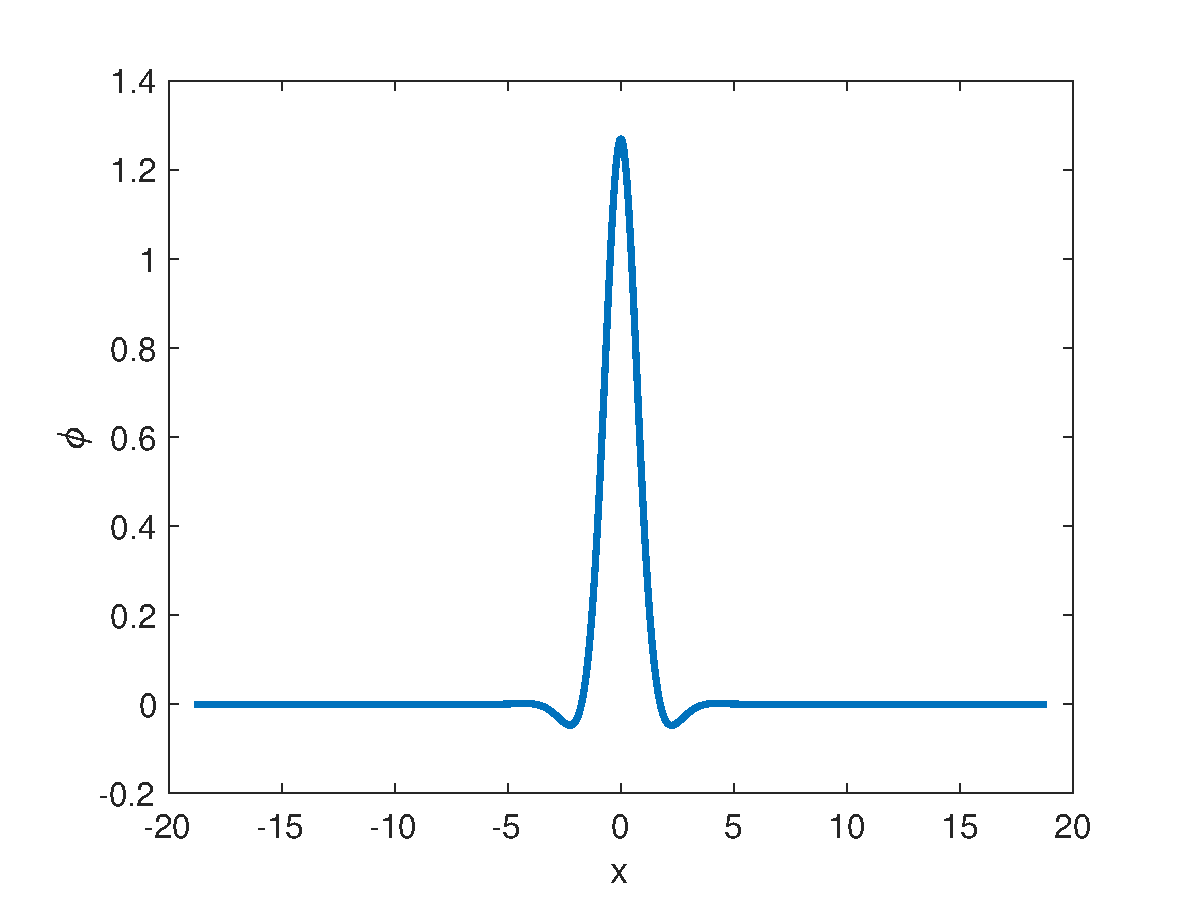
\includegraphics[width=8cm]{images/PQS1.eps} &
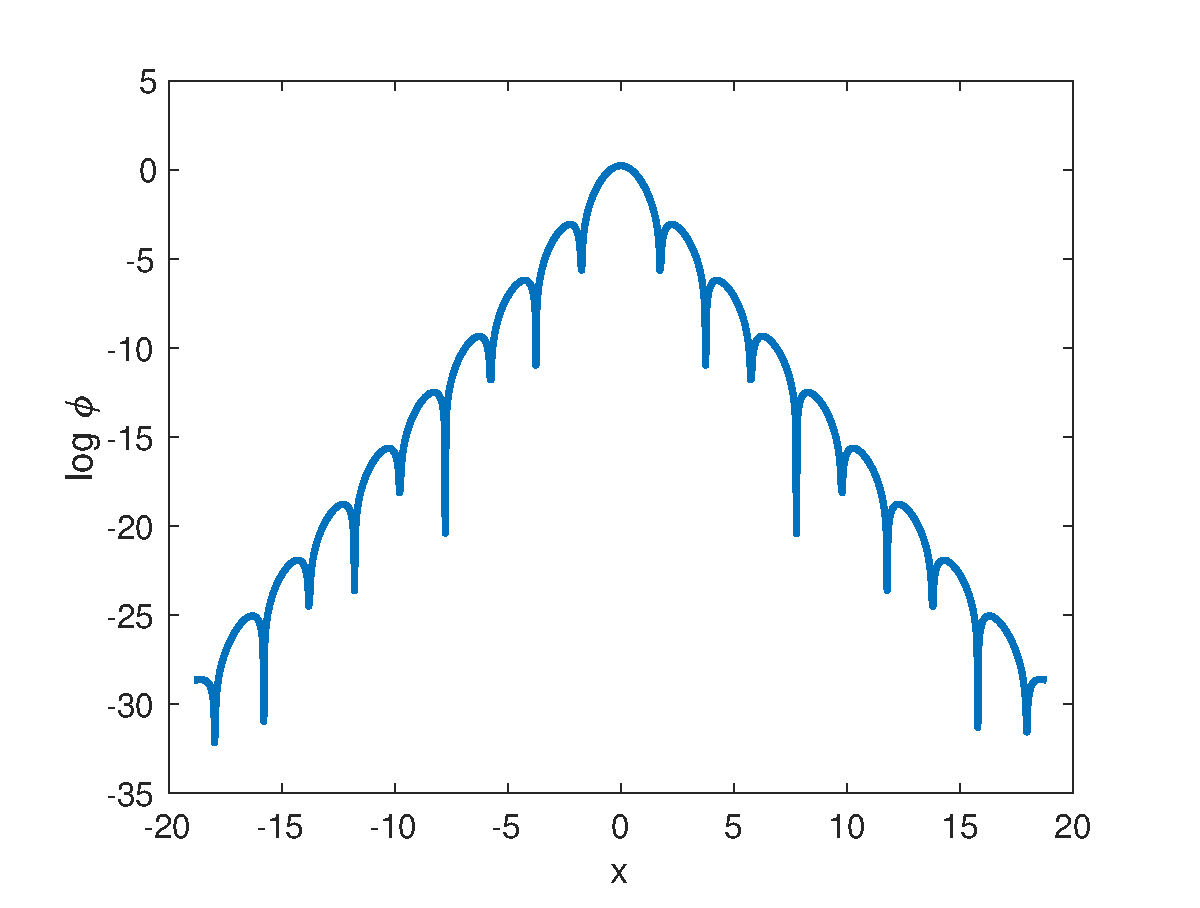
\includegraphics[width=8cm]{images/PQS1log.eps}
\end{tabular}
\caption{Pure quartic solitary wave solution $\phi(x)$ to \cref{standingwavereal} with $\beta_2 = 0$, $\beta_4 = -1$, $\omega = 1$. (left panel). Plot of $\log \phi(x)$ vs $x$ (right panel) showing exponentially-decaying oscillatory tails. }
\label{fig:PQS}
\end{figure} 

\begin{figure}[H]
\centering
\begin{tabular}{cc}
\includegraphics[width=8cm]{images/PQSspec.eps} &
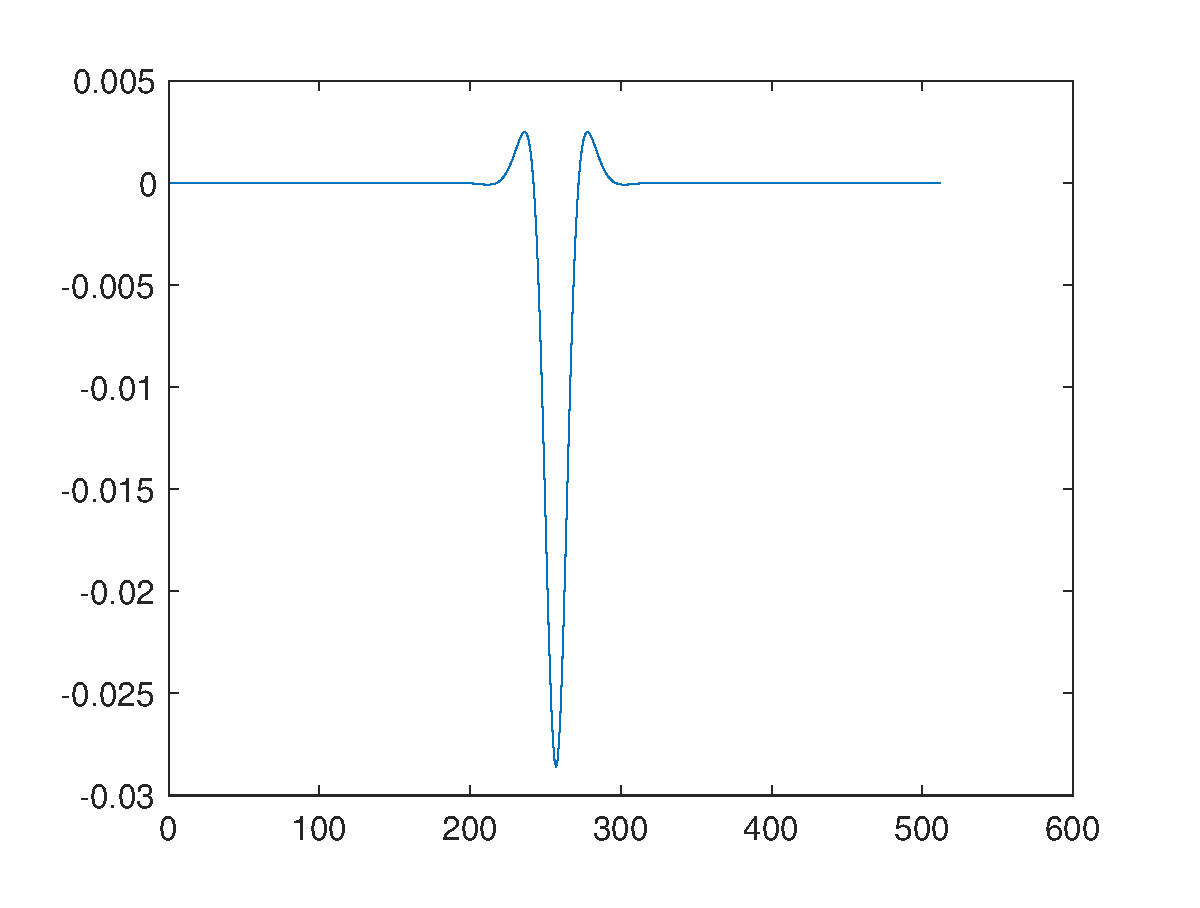
\includegraphics[width=8cm]{images/PQSinternalmode.eps}
\end{tabular}
\caption{Spectrum of pure quartic solitary wave (left panel), $\beta_2 = 0$, $\beta_4 = -1$, $\omega = 1$. Kernel eigenvalues in black, internal mode eigenvalues in red. Eigenvalues in blue correspond to the discrete essential spectrum. Eigenfunction corresponding to internal mode eigenvalues (right panel).}
\label{fig:PQSspec}
\end{figure} 

For the single pulse solitary wave solutions, we can compute the stability criterion \cref{ddoubleprime} from \cite{Grillakis1987}. In all cases, $M = d''(\omega) > 0$ (for example for $\beta_4 = -1, \beta_2 = 0, \omega = 1$, $d''(\omega) = 0.7291$), thus numerical results suggest that primary pulse solution is orbitally stable. In addition, numerical computation suggests that $\tilde{M} > 0$.

To construct double pulses, we glue together two copies of the primary pulse at the pulse distances predicted by \cref{theorem:multiexist} and solve for the double pulse solution using the same Newton conjugate-gradient method. The first eight double pulse solutions are shown in \cref{fig:doublepulses}. Arbitrary multi-pulses can similarly be constructed.

\begin{figure}[H]
\centering
\begin{tabular}{cc}
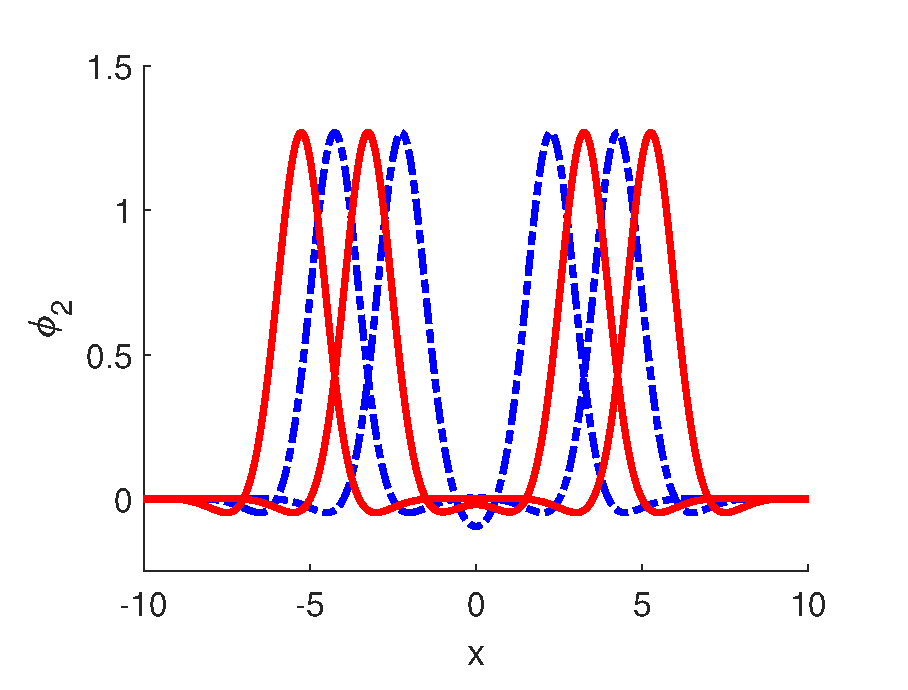
\includegraphics[width=8cm]{images/DPplus.eps} &
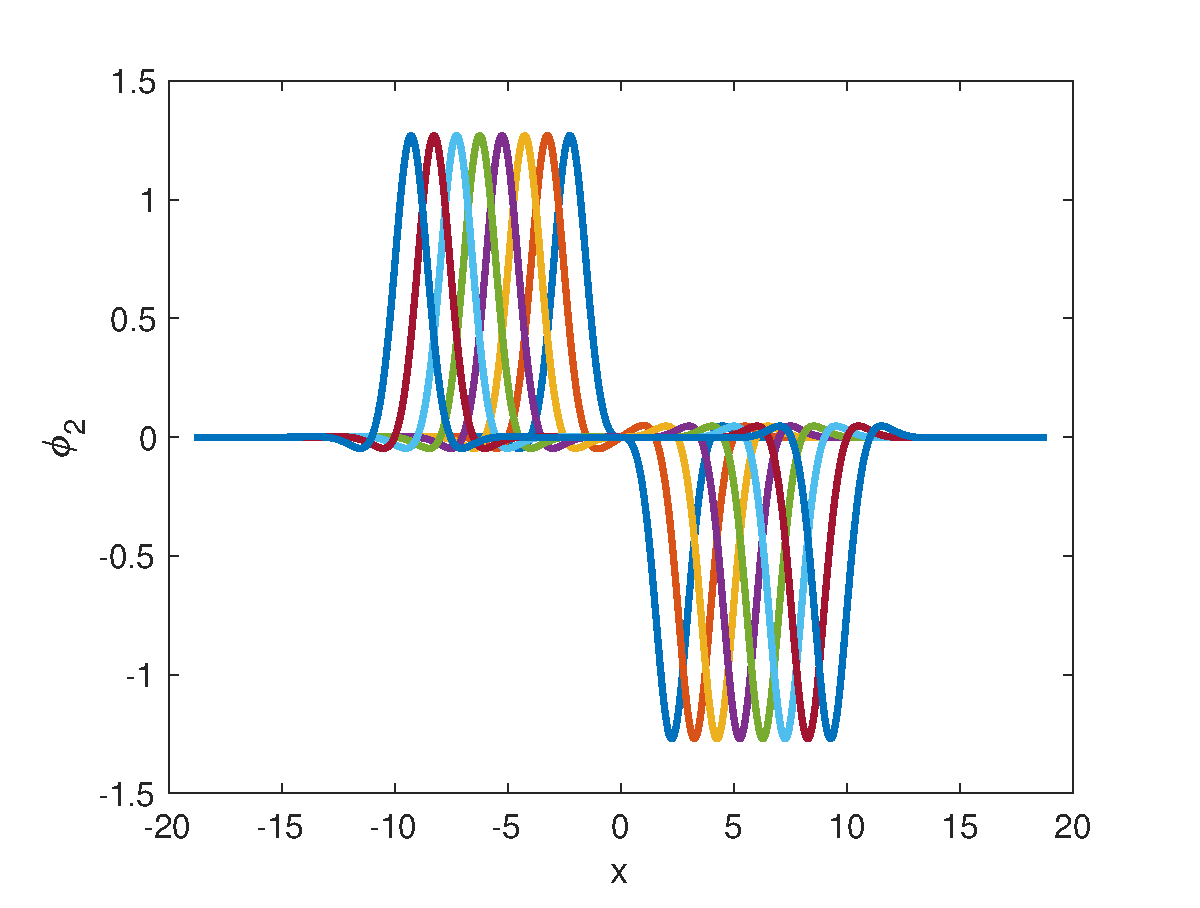
\includegraphics[width=8cm]{images/DPminus.eps}
\end{tabular}
\caption{First eight double pulse solutions $\phi_2(x)$ constructed from two pure quartic solitary wave solution $\phi(x)$ to \cref{standingwavereal} with $\beta_2 = 0$, $\beta_4 = -1$, $\omega = 1$. In-phase double pulses (left panel), opposite phase double pulses (right panel). }
\label{fig:doublepulses}
\end{figure} 

To determine the spectrum of the linearization about the double pulse solutions, we construct the linear operator $\calL(\phi_2)$ using Fourier spectral differentiation matrices and compute the eigenvalues using Matlab's eigenvalue solver \texttt{eig}. In all cases, there is a pair of purely imaginary interaction eigenvalues and a pair of real interaction eigenvalues, thus the double pulses are all unstable (\cref{fig:doublespec}). There is also a duplication of the internal mode eigenvalues (\cref{fig:doubleinternalmode}). Since in all cases there is an eigenvalue with positive real part, the duplication of internal mode eigenvalues does not affect stability. 

\begin{figure}[H]
\centering
\begin{tabular}{cc}
\includegraphics[width=8cm]{images/inteigsDP1plus.eps} &
\includegraphics[width=8cm]{images/inteigsDP1plus.eps}
\end{tabular}
\caption{Eigenvalues for first in-phase double pulse (left panel) and first out-of-phase double pulse (right panel). Interaction eigenvalues shown in red, and kernel eigenvalues in black. Eigenvalues in blue correspond to the discrete essential spectrum; as expected, these eigenvalues are on the imaginary axis and have magnitude $|\lambda| \geq \omega$. Internal mode eigenvalues are not shown. $\beta_2 = 0$, $\beta_4 = -1$, $\omega = 1$.}
\label{fig:doublespec}
\end{figure} 

\begin{figure}[H]
\centering
\begin{tabular}{c}
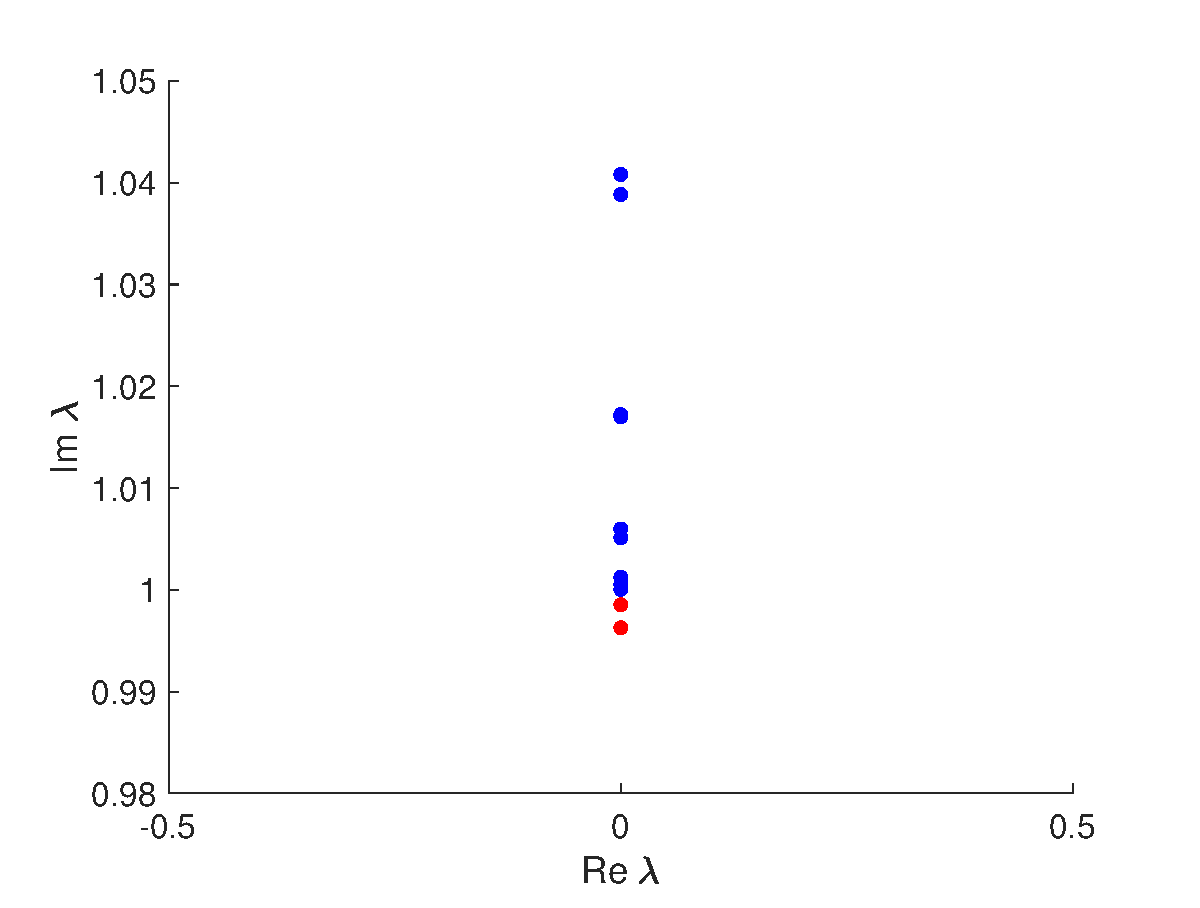
\includegraphics[width=8cm]{images/DP3internalmode.eps}
\end{tabular}
\caption{Close-up of spectrum showing pair of internal mode eigenvalues (red) and eigenvalues corresponding to the essential spectrum (blue) for third in-phase double pulse. $\beta_2 = 0$, $\beta_4 = -1$, $\omega = 1$.}
\label{fig:doubleinternalmode}
\end{figure}

Finally, \cref{fig:inteigpred} plots the log of the relative error for the eigenvalues $\lambda_\pm$ between the value computed by Matlab's eigenvalue solver \texttt{eig} and that given by the leading order term in the formula \cref{inteigpred} versus the pulse separation distance $X$. The error decreases as $X$ increases, as predicted. 

\begin{figure}[H]
\centering
\begin{tabular}{c}
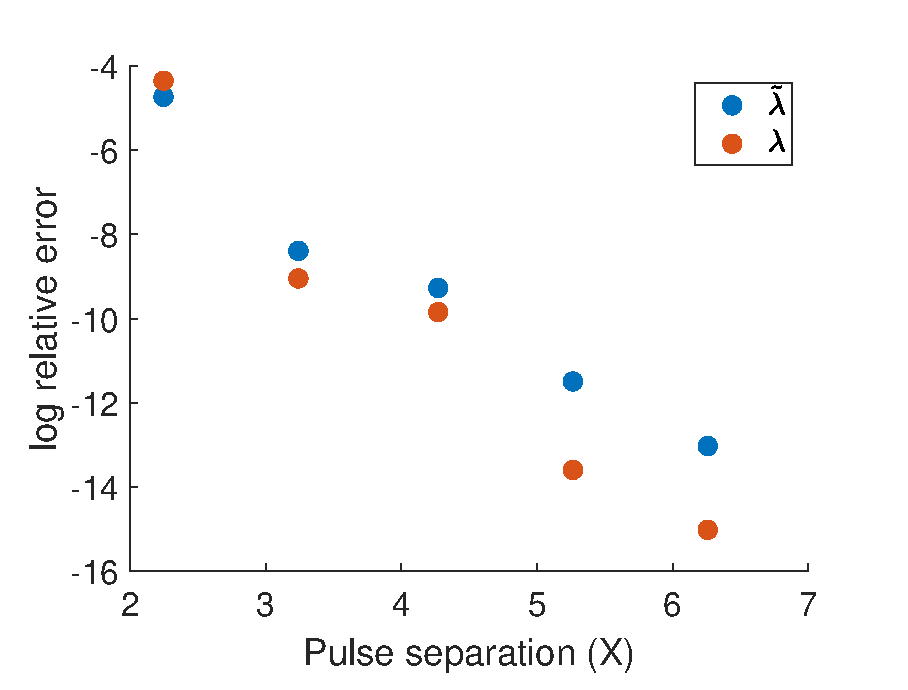
\includegraphics[width=8cm]{images/inteigpred.eps}
\end{tabular}
\caption{Log of the relative error for the eigenvalues $\lambda_\pm$ versus the pulse separation $X$ for the first five in-phase double pulses. $\beta_2 = 0$, $\beta_4 = -1$, $\omega = 1$.}
\label{fig:inteigpred}
\end{figure}

\appendix

\section{Proof of stability results}

\subsection{Proof of Theorem \ref{th:blockmatrix}}\label{sec:blockmatrixproof}

The proof is adapted from \cite{Manukian} and \cite{Sandstede1998}. Let $U(x)$ be the primary pulse solution, with first component $\phi(x)$. Let $U_n(x)$ be be an $n$-modal solution to \cref{Fsystem} constructed according to \cref{theorem:multiexist} with phase parameters $\theta_1, \dots, \theta_n \in \{ -1, 1 \}^n$ and pulse separation distances $X_1, \dots, X_{n-1}$ given by \cref{pulsedistances}. Let $\phi_n(x)$ be the first component of $U_n(x)$, and write $U_n(x)$ in piecewise form as \cref{Unpiecewise}. The eigenvalue problem associated with the multi-pulse $U_n$ is given by \cref{multieig}, with $\phi_n$ in place of $\phi$. It follows from \cref{Lphikernel} that
\begin{equation}\label{Kkernel}
\begin{aligned}
[Y(x)]' &= K(\phi_n)Y(x), \quad [Z(x)]' = K(\phi_n)Z(x) + B_1 Y(x) \\
[\tilde{Y}(x)]' &= K(\phi_n)\tilde{Y}(x), \quad [\tilde{Z}(x)]' = K(\phi_n)\tilde{Z}(x) + B_1 \tilde{Y}(x)
\end{aligned}
\end{equation}
where
\begin{equation}
\begin{aligned}
Y(x) &= ( 0, U_n(x) )^T, \quad
Z(x) = ( \partial_\omega U_n(x), 0 )^T \\
\tilde{Y}(x) &= ( \partial_x U_n(x), 0)^T, \quad
\tilde{Z}(x) = ( 0, Z_n(x) )^T,
\end{aligned}
\end{equation}
and $Z_n(x) = (z_n(x), \partial_x z_n(x), \partial_x^2 z_n(x), \frac{\beta_4}{24} \partial_x^3 z_n(x))$, where the first component $z_n(x)$ solves $\calL^-(\phi_n)z_n = \phi_n'$. The analysis is identical to that of \cite{Manukian}, except the piecewise ansatz for the eigenfunction also involves $Z(x)$ and $\tilde{Z}(x)$. Writing the functions \cref{Kkernel} in piecewise form as with \cref{Unpiecewise}, we will use the ansatz
\begin{align}\label{Vansatz}
V_i^\pm(x)' &= d_i(Y_i^\pm(x) + \lambda Z_i^\pm(x)) + \tilde{d}_i(\tilde{Y}_i^\pm(x) + \lambda \tilde{Z}_i^\pm(x)) + W_i^\pm && i = 1, \dots, n.
\end{align}
Substutiting this into \cref{multieig} and simplifying using \cref{Kkernel}, the remainder functions $W_i^\pm(x)$ solve the equation
\begin{align}\label{Wsolves}
W_i^\pm(x)' &= K(\phi_n)W_i^\pm(x) + \lambda^2 d_i B Z_i^\pm(x) + \lambda^2 \tilde{d}_i B \tilde{Z}_i^\pm(x) && i = 1, \dots, n
\end{align}
Following \cite{Manukian,Sandstede1998}, we obtain a unique piecewise solution $W_i^\pm(x)$ which generically has $n$ jumps at $x = 0$ in the direction of $Q^*(0) \oplus \tilde{Q}^*(0)$. Using the definitions of $Q^*(x)$ and $\tilde{Q}^*(x)$ together with \cref{Unestimates} and \cite[(3.19)]{Manukian}, these jumps are given by
\begin{equation}\label{jumpcond1}
\begin{aligned}
\xi_i &= \theta_{i+1} \langle \Psi(X_i), U(-X_i) \rangle (d_{i+1} - d_i) 
+ \theta_{i-1} \langle \Psi(-X_{i-1}), U(X_{i-1}) \rangle (d_i - d_{i-1} )  \\
&\qquad + \lambda^2 \theta_i d_i \int_{-\infty}^\infty \langle \Psi(y), B \partial_\omega U(y) \rangle dy 
+ \mathcal{O}((|\lambda| + e^{-\alpha X_{\min}})^3) \\
\tilde{\xi}_i &= \theta_{i+1} \langle \Psi'(X_i), U'(-X_i) \rangle (\tilde{d}_{i+1} - \tilde{d}_i) 
+ \theta_{i-1} \langle \Psi'(-X_{i-1}), U'(X_{i-1}) \rangle (\tilde{d}_i - \tilde{d}_{i-1}) \\
&\qquad- \lambda^2 \theta_i \tilde{d}_i \int_{-\infty}^\infty \langle \Psi(y), B Z(y) \rangle dy 
+ \mathcal{O}((|\lambda| + e^{-\alpha X_{\min}})^3),
\end{aligned}
\end{equation}
where $Z(x) = (z(x), \partial_x z(x), \partial_x^2 z(x), \frac{\beta_4}{24} \partial_x^3 z(x))$. By symmetry, 
\begin{equation}\label{Rrelation}
\Psi(-x) = -R \Psi(x), \quad U(-x) = R U(x),
\end{equation}
where $R$ is the standard reversor operator 
\[
R(u_1, u_2, u_3, u_4) = (u_1, -u_2, u_3, -u_4),
\] 
thus 
\begin{align*}
\langle \Psi(-X_{i-1}), U(X_{i-1}) \rangle &= -\langle \Psi(X_{i-1}), U(-X_{i-1}) \rangle \\
\langle \Psi'(-X_{i-1}), U'(X_{i-1}) \rangle &= -\langle \Psi'(X_{i-1}), U'(-X_{i-1}) \rangle.
\end{align*} 

Finally, we relate $\Psi(X_i), U(-X_i) \rangle$ and $\Psi'(X_i), U'(-X_i) \rangle$. Since $DF(\phi) = K^+(\phi)$, $\Psi(x)$ is the unique bounded solution to the adjoint equation $W'(x) = -DF(\phi)^* W(x)$. Thus by \cite[Lemma 6.1]{Sandstede1998} and the reversibility relations \cref{Rrelation}, with $\Psi'(x)$ in place of $\Psi(x)$, $p$ in place of $\phi$, and no dependence on a parameter $\mu$,
\begin{align}
\langle \Psi'(x), U(-x) &= \langle \Psi'(-x), U(x) \rangle = s e^{-2 a x} \sin(2 b x + p) + \mathcal{O}(e^{-(2 \alpha + \gamma)x}) \label{IPdPsiU} \\
\langle \Psi'(x), U'(-x) \rangle &= 
\langle \Psi'(x), U'(-x) \rangle = -s e^{-2 a x} \left( b \cos(2 b x + p) - a \sin(2 b x + p) \right) + \mathcal{O}(e^{-(2 \alpha + \gamma)x}) \label{IPdPsidU}
\end{align}
where $s > 0$ and $\gamma > 0$. Differentiating $\langle \Psi(-x), U(x) \rangle$ with respect to $x$, since the operator $\partial_x$ is skew symmetric, 
\begin{align*}
\frac{d}{dx} \langle \Psi(x), U(-x) \rangle = 2 \langle \Psi'(x), U(-x) \rangle,
\end{align*}
thus we can integrate \cref{IPdPsiU} by parts to get 
\begin{align*}
\langle \Psi(x), U(-x) \rangle = -\frac{1}{a^2 + b^2} s e^{-2 a x} \left( b \cos(2 b x + p) + a \sin(2 b x + p) \right) + \mathcal{O}(e^{-(2 \alpha + \gamma)x}).
\end{align*}
In the proof of \cite[Theorem 3]{Sandstede1998}, the distances $X_i$ are chosen to solve $s e^{-2 a X_i} \sin(2 b X_i + p) = \mathcal{O}(e^{-(2 \alpha + \gamma)X_i})$, thus for $X = X_i$ we have
\begin{align}\label{IPrelation1}
\langle \Psi'(x), U'(-x) \rangle = (a^2 + b^2)
\langle \Psi(x), U(-x) \rangle
\end{align}
Using \cref{IPrelation1}, multiplying by $\theta_i$ and using the definition of $B$, equations \cref{jumpcond1} simplify to the jump conditions
\begin{align*}
\xi_i &= \theta_i \theta_{i+1} \langle \Psi(X_i), U(-X_i) \rangle (d_{i+1} - d_i) 
- \theta_{i-1} \theta_i  \langle \Psi(X_{i-1}), U(-X_{i-1}) \rangle (d_i - d_{i-1}) \\
&\qquad + \lambda^2 d_i \int_{-\infty}^\infty \phi(y) \partial_\omega \phi(y) dy 
+ \mathcal{O}( |\lambda|(|\lambda| + e^{-\alpha X_{\min}})^2 + e^{-(2 \alpha + \gamma)X_{\min} }) )  \\
\tilde{\xi}_i &= (a^2 + b^2) \theta_i \theta_{i+1} \langle \Psi(X_i), U(-X_i) \rangle (\tilde{d}_{i+1} - \tilde{d}_i)
- (a^2 + b^2) \theta_{i-1} \theta_i \langle \Psi(X_{i-1}), U(-X_{i-1}) \rangle (\tilde{d}_i - \tilde{d}_{i-1}) \\
&\qquad- \lambda^2 \tilde{d}_i \int_{-\infty}^\infty \partial_y \phi(y) z(y) dy
+ \mathcal{O}( |\lambda|(|\lambda| + e^{-\alpha X_{\min}})^2 + e^{-(2 \alpha + \gamma)X_{\min} }) ) ,
\end{align*}
which we write in matrix form as in the statement of the theorem.

\subsection{Proof of Corollary \ref{corr:multiunstable} and Corollary \ref{corr:2pstab}}

For \cref{corr:multiunstable}, let $\{ \mu_1,\dots,\mu_{n-1}, 0\}$ be the eigenvalues of $A$, which are real and distinct by the proof of \cite[Theorem 5]{Parker2020}. Following the steps in that proof and using the rescaling in \cite[Theorem 3]{Sandstede1998}, there are $2(n-1)$ pairs of interaction eigenvalues, given by \cref{inteigs}, which are either real or purely imaginary by Hamiltonian symmetry. Since $M > 0$ by \cref{hyp:dccpos}, if $\tilde{M} > 0$ as well, then one of each pair $\lambda_i, \tilde{\lambda}_i$ is real and the other is purely imaginary. \cref{corr:2pstab} is the specific case $n = 2$, where the nonzero eigenvalue of $A$ can be computed directly.

% \bibliographystyle{amsalpha}
\bibliography{NLS4.bib}

\end{document}